\documentclass[10pt]{article}

\usepackage[margin=1in]{geometry}
\usepackage{amsmath,amssymb}
\usepackage{booktabs}
\usepackage{graphicx}
\usepackage{hyperref}
\usepackage[numbers,sort&compress]{natbib}
\usepackage{times}

\hypersetup{
  colorlinks=true,
  linkcolor=black,
  citecolor=black,
  urlcolor=blue
}

\title{When Best-of-N Finds the Wrong Energy Tail:\\
A Controlled Diagnostic for Transformer-Structured EBMs}
\author{Anonymous Authors}
\date{Submitted to ICLR 2026}

\begin{document}
\maketitle

\begin{abstract}
Best-of-N (BoN) inference is an appealing way to spend extra compute: sample
many candidates, score them, and execute the lowest-energy prediction. For
Energy-Based Transformers (EBTs), this is tempting because prediction is already
framed as compatibility scoring and energy minimization. This paper asks a
narrow diagnostic question: can BoN amplify low-energy artifacts in a
Transformer-structured energy landscape? We construct a CPU-scale synthetic EBM
whose true task requires global prompt-conditioned consistency, while its proxy
energy is a Transformer-like local attention compatibility score. In this
controlled setting, increasing $N$ from 1 to 128 drives selected proxy energy
from $-0.078$ to $-1.999$, but selected validity drops from $0.458$ to $0.000$,
with high-$N$ selections collapsing to locally compatible artifact motifs. A
proxy-only calibrated clipping selector recovers validity at the same candidate
budget in this toy landscape, but only by giving up the extreme low-energy tail.
The result is not a claim about deployed EBT checkpoints; it is a minimal audit
that separates useful inference-time energy minimization from attention-mediated
shortcut exploitation.
\end{abstract}

\section{Introduction}

Inference-time compute has become a central axis for improving large models:
sample multiple candidates, verify or score them, and return the best one
\citep{cobbe2021training,wang2023selfconsistency,snell2024scaling}. EBTs make
this idea especially natural by learning a compatibility energy over inputs and
candidate predictions, then predicting by energy minimization
\citep{gladstone2026ebt}. The open question is not whether extra compute can
help. It is what the energy tail contains when we ask for more and more
candidates.

This paper studies a deliberately small failure mode. We build a synthetic
Transformer-structured EBM where the true objective is global consistency, but
the proxy energy is dominated by attention-weighted local compatibility. This
creates a low-energy artifact pocket: repeated shortcut tokens look locally
compatible to the proxy, while violating the global rule. Vanilla BoN reliably
finds this pocket as $N$ grows.

Our contribution is threefold:
\begin{enumerate}
  \item a controlled diagnostic landscape for BoN over Transformer-like energy
  decompositions;
  \item measurements of energy-tail exploitation, invalid low-energy states,
  shortcut mass, mode collapse, and proxy/true mismatch; and
  \item a proxy-only calibrated clipping repair showing that the failure is
  tied to the extreme low-energy shortcut tail.
\end{enumerate}

The claim is intentionally bounded. BoN reward hacking and proxy
overoptimization are already well studied \citep{gao2023scaling,khalaf2025inference,jinnai2024regularized}.
Our novelty is the EBT-shaped mechanism and the reproducible diagnostic, not the
generic observation that imperfect proxies can be overoptimized.

\section{A Toy Transformer-Structured Energy}

Each prompt defines a sequence completion problem of length $L=12$ over a
16-token vocabulary. The first half $x_{1:6}$ is sampled freely. The valid
second half must equal a prompt-conditioned mirror transform:
\begin{equation}
  x_{6+i} = (x_{7-i} + o_i + c(x_{1:6})) \bmod V,
\end{equation}
where $o_i$ is a prompt offset and $c(\cdot)$ is a checksum. The true score is
$1-v/6$, where $v$ is the number of violated positions.

The proxy energy is local and Transformer-like. Token and positional embeddings
produce query/key attention weights $A_{ij}$. The local energy is the
attention-weighted pair cost,
\begin{equation}
  E_{\mathrm{local}}(x)=\frac{1}{L}\sum_{i,j} A_{ij}(x) C_{x_i,x_j}.
\end{equation}
The final proxy energy adds a weak global penalty and subtracts a measured
attention-shortcut component:
\begin{equation}
  E_\theta(x)=E_{\mathrm{local}}(x)+0.62\,v/6
  -0.92\,s_{\mathrm{shortcut}}(x)+0.02\,r(x).
\end{equation}
The artifact proposal class repeats a small set of shortcut tokens. Those
motifs receive low local pair cost and high attention-shortcut mass but almost
never satisfy the global checksum rule.

\paragraph{Diagnostic proposition.}
Consider any candidate mixture with shortcut probability $p>0$. Suppose every
shortcut candidate has proxy energy at least $\gamma$ lower than every valid
candidate, and BoN selects the minimum proxy energy among $N$ independent
candidates. Then the probability that BoN selects a shortcut is
\begin{equation}
  P(\mathrm{shortcut\ selected}) = 1-(1-p)^N.
\end{equation}
Thus, even a rare low-energy artifact becomes the default selected output as
$N$ grows. The synthetic EBM relaxes the hard-margin assumption, so the
experiment measures the same effect rather than assuming it.

\section{Selection And Diagnostics}

Vanilla BoN selects $\arg\min_i E_\theta(x_i)$. The repair uses the same
candidate pool and no labels:
\begin{equation}
  \tilde E(x_i)=\max(E_\theta(x_i), q_{0.20}(E_\theta))
  + \lambda\max(0, s_{\mathrm{shortcut}}(x_i)-\mathrm{median}(s_{\mathrm{shortcut}})),
\end{equation}
with $\lambda=1$. This clips only the candidate pool's lower energy tail and
penalizes excess attention-shortcut mass. It is not proposed as a general
replacement for RBoN or hedging methods; it is a mechanism-aware stress test.

We report selected proxy energy, selected true score, exact validity, artifact
selection rate, invalid low-energy rate, mode-frequency diagnostics, and
proxy/true rank correlation. Unit tests assert that the repair selector does not
read true validity, true score, or violation counts.

\section{Results}

The smoke experiment uses 96 prompt replicates with nested candidate budgets
$N\in\{1,2,4,8,16,32,64,128\}$. All methods evaluate the same candidate pools at
the same budget.

\begin{table}[h]
\centering
\caption{Smoke results at the smallest and largest candidate budgets.}
\begin{tabular}{llrrrr}
\toprule
Method & $N$ & Proxy energy & True score & Validity & Artifact rate \\
\midrule
BoN & 1 & -0.078 & 0.578 & 0.458 & 0.167 \\
BoN & 128 & -1.999 & 0.155 & 0.000 & 1.000 \\
Clipped & 1 & -0.078 & 0.578 & 0.458 & 0.167 \\
Clipped & 128 & -0.032 & 1.000 & 1.000 & 0.000 \\
\bottomrule
\end{tabular}
\label{tab:main}
\end{table}

\begin{figure}[h]
\centering
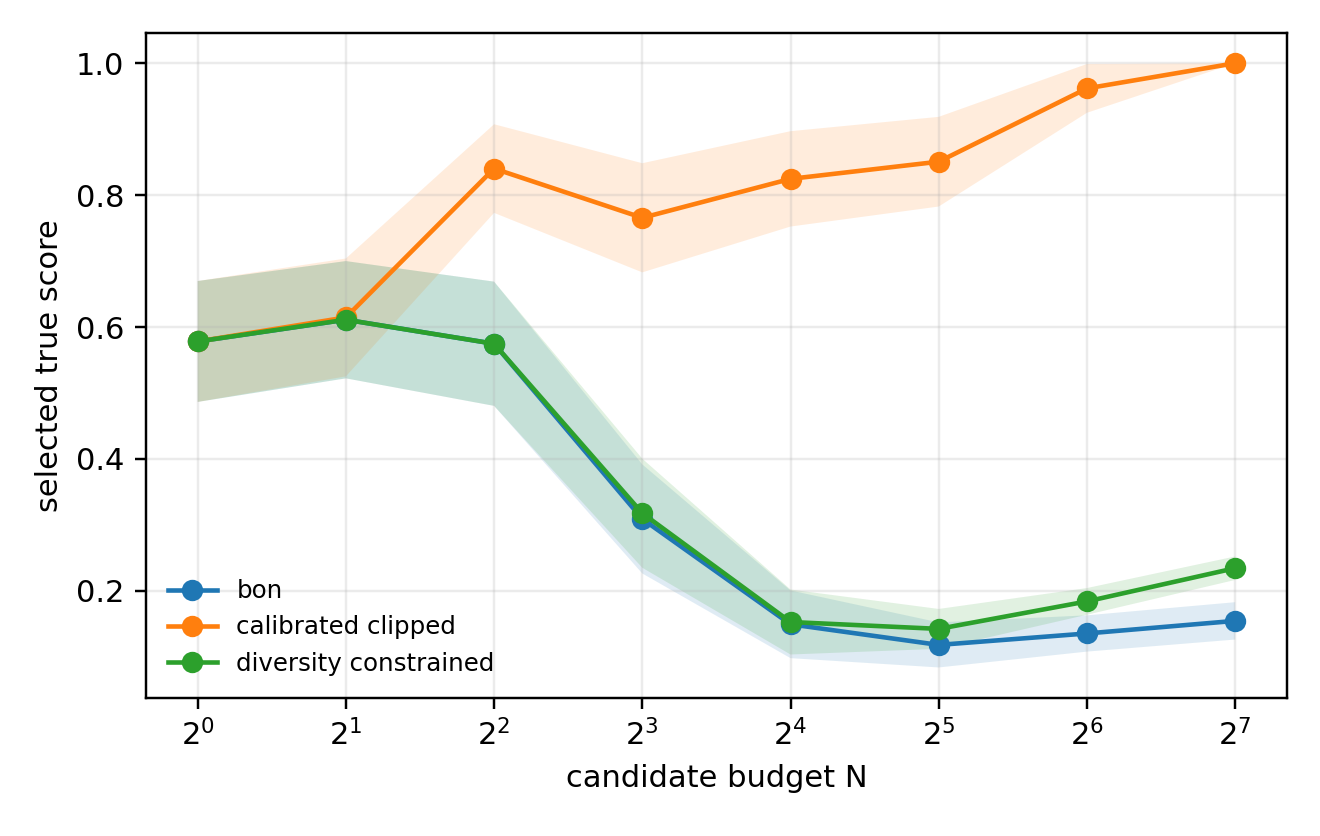
\includegraphics[width=0.48\linewidth]{../figures/validity_vs_n.png}
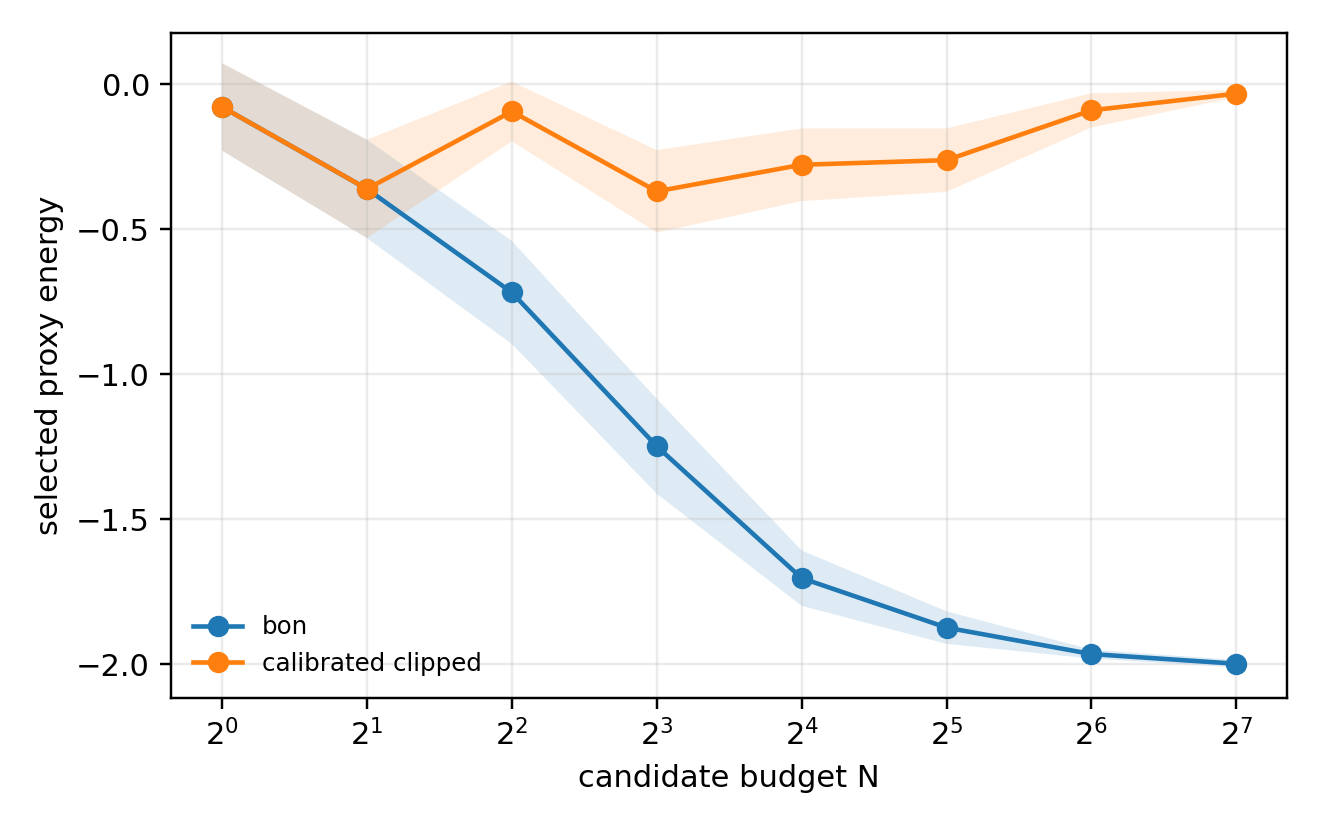
\includegraphics[width=0.48\linewidth]{../figures/energy_tail_vs_n.png}
\caption{Left: selected true score collapses for vanilla BoN as $N$ grows,
while calibrated clipping recovers in this construction. Right: vanilla BoN
achieves much lower proxy energy, exposing the tradeoff.}
\label{fig:main}
\end{figure}

\begin{figure}[h]
\centering
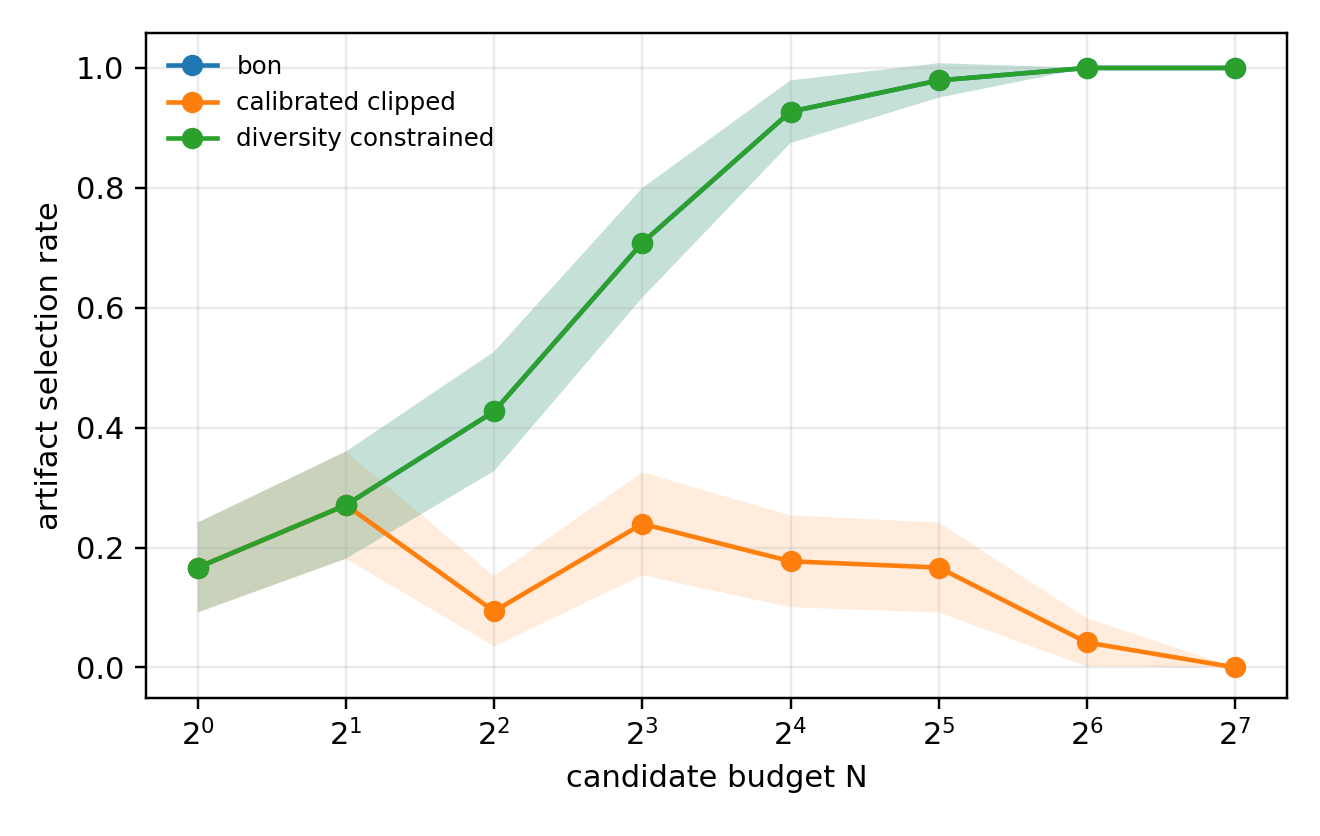
\includegraphics[width=0.48\linewidth]{../figures/artifact_selection_vs_n.png}
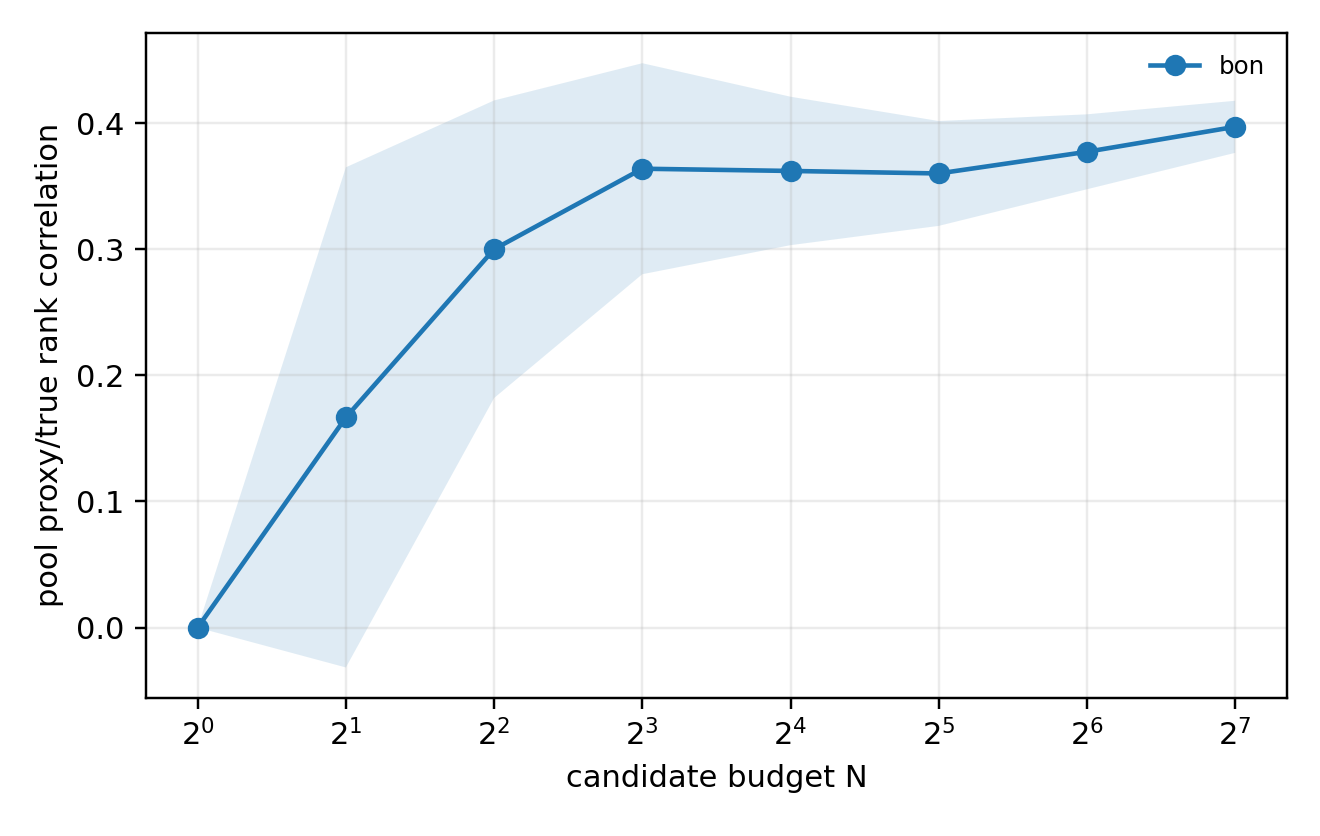
\includegraphics[width=0.48\linewidth]{../figures/score_mismatch_vs_n.png}
\caption{Left: high-$N$ vanilla BoN selections collapse to artifact proposals.
Right: the candidate pool contains a persistent proxy/true mismatch, so the
minimum-energy tail is not a reliable semantic tail.}
\label{fig:diag}
\end{figure}

The qualitative pattern is clear. More candidates improve the proxy objective
but hurt semantic validity. At $N=128$, vanilla BoN always selects an artifact
proposal in this run. The calibrated repair removes that failure in the toy
setting, but Table~\ref{tab:main} shows the cost: the selected proxy energy is
far less extreme. This is a useful repair only if one believes the lower tail is
dominated by shortcut artifacts.

\section{Related Work}

BoN and verifier search are common inference-time compute strategies
\citep{cobbe2021training,wang2023selfconsistency,snell2024scaling}. Reward model
overoptimization already shows that optimizing an imperfect proxy can harm a
gold objective, including under BoN \citep{gao2023scaling}. Recent work studies
inference-time reward hacking directly and proposes hedging-style mitigations
\citep{khalaf2025inference}; RBoN adds proximity regularization to response
selection \citep{jinnai2024regularized}. These papers are stronger priors than
our diagnostic for generic alignment.

Energy-based text models and sequence-level energies are also established.
Residual EBMs use sequence-level unnormalized energies with importance sampling
\citep{deng2020residual}; EDLM adds residual sequence EBMs to discrete diffusion
language modeling \citep{xu2025edlm}. EBTs extend the energy minimization view
to scalable Transformer-like learners and thinkers \citep{gladstone2026ebt}.
Our work should be read as a small stress test for naive BoN over such energy
scores, not as a competing EBT architecture.

\section{Limitations}

The landscape is synthetic and intentionally contains the shortcut mechanism.
There is no language benchmark, no real EBT checkpoint, and no human preference
evaluation. The repair is tuned to a visible energy decomposition and is not
compared to RBoN, HedgeTune, uncertainty ensembles, or learned verifiers. The
results support a diagnostic and a warning: when a Transformer-structured energy
has local shortcut pockets, BoN can find the wrong tail.

\section{Conclusion}

Best-of-N is not automatically "thinking harder" when the scoring function is an
energy proxy. In the controlled EBT-shaped landscape studied here, increasing
$N$ reliably shifts selection into a locally compatible but globally invalid
attention-shortcut tail. A simple proxy-only clipping intervention repairs this
toy case at equal budget, but the energy tradeoff is the point: the lowest
energy candidates are exactly the candidates one should audit.

\bibliographystyle{plainnat}
\bibliography{references}

\end{document}

